\suppnote{Joint-spectrum, daily-score and coherent-response results}{note:spectral-results}

The joint field spectra, daily P/D scores and coherent response answer different questions. No operator is refitted for the spectral displays. The coherent comparison uses the same per-date DFT support as the joint spectrum in each city.

\paragraph{Three-city joint spectra.} At the eight-mode display cut in Figure~\ref{fig:supp-1}, source energy coverage is 0.6343, 0.9656 and 1.0000 in Porto, San Francisco and Chengdu, and routing coverage is 0.7989, 0.9892 and 1.0000. Chengdu's complete coverage follows from its eight-TRAIN-date snapshot-rank ceiling and does not demonstrate greater intrinsic low dimensionality. The common logarithmic floor is $10^{-4.5}$; all displayed cells exceed it. Chengdu's time-independent component carries 0.668 of source energy and 0.811 of full-face routing energy. The weighted spectra account for raw-block energy to machine precision; this is a numerical conservation check, not held-out evidence.

\paragraph{Held-out daily P/D scores.} Figure~\ref{fig:supp-2} resolves the pooled entries in Table~\ref{tab:crosscity} by TEST date. Porto has 51 TEST dates, San Francisco has five blocked folds and Chengdu has three TEST dates in the continuous-observation protocol. The daily spread is descriptive: it does not replace the common pooled-error convention and does not supply the missing paired-date interval for the primary D comparison. In particular, Chengdu's three dates are insufficient for a strong date-heterogeneity claim.

\paragraph{Coherent TRAIN/TEST response.} Figure~\ref{fig:supp-3} compares the frozen P-selected operator with observed coherent routing on both TRAIN and TEST. TRAIN panels describe the fit sample and are not independent validation. On TEST, the direction alignments $\gamma_m$ at $m=0$ are 0.978, 0.943 and 0.821 in Porto, San Francisco and Chengdu, respectively; at the first nonzero bin $m=1$ they are 0.935, 0.908 and 0.628. The corresponding norm ratios $\rho_m$ are 0.800, 0.612 and 0.709 at $m=0$, and 0.790, 0.849 and 0.596 at $m=1$. San Francisco values are fold means. Across all ten Chengdu bins, alignment spans 0.474--0.821 and norm ratio spans 0.596--0.747. These results show partial alignment in both direction and magnitude; they do not convert coherent-date averages into observation-level P/D scores.

\begingroup\sloppy
\paragraph{Underpowered Chengdu full-FACE nonlinear exploration.} Figure~\ref{fig:supp-7} reports an exploratory 18-phase A-to-D comparison on the complete FACE target. For each nonlinear arm, $\Delta R^2$ is the mean-date full-FACE error of \texttt{linF} minus that of the arm, so positive values favour the nonlinear arm. The \texttt{quadF} contrast is $-0.005854$ with descriptive 95\% interval $[-0.006105,-0.005661]$; the \texttt{krrF} contrast is $+0.000418$ with interval $[-0.000023,+0.000698]$, which crosses zero.

There are only three TEST dates, and D's all-phase linear design has 144 columns for 144 TRAIN rows and is therefore saturated.

The design is \textbf{underpowered}: these arms neither establish a nonlinear improvement nor support a claim of no nonlinearity.

Full-FACE scores must not be mixed with POD-internal scores. Although 9,999 paired-date bootstrap draws are recorded, three dates provide only 27 ordered date resamples, so the intervals are descriptive rather than confirmatory.

\endgroup

\begin{figure}[!htbp]
\centering
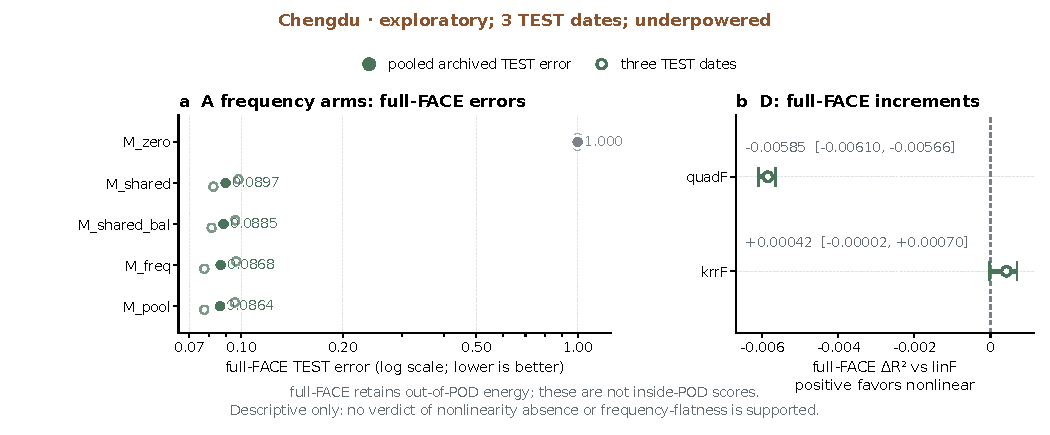
\includegraphics[width=0.74\textwidth]{figures_supp/figS07_nonlinear_exploratory.pdf}
\caption{\textbf{Underpowered exploratory Chengdu full-FACE nonlinear comparison.} Full-FACE $\Delta R^2$ relative to \texttt{linF} for \texttt{quadF} and \texttt{krrF} on the 18-phase A-to-D design, with descriptive 95\% paired-date intervals. \texttt{quadF} gives $-0.005854$ $[-0.006105,-0.005661]$; \texttt{krrF} gives $+0.000418$ $[-0.000023,+0.000698]$. Only three TEST dates are available, and the 144-column linear design saturates the 144 TRAIN rows. The experiment is exploratory and underpowered; it does not demonstrate either the presence or absence of nonlinearity.}
\label{fig:supp-7}
\end{figure}
